	Ein \emph{(polygonaler) Kantenzug} $P = (p_1, p_2, \mathellipsis, p_n)$ ist eine Aneinanderreihung von Geradensegmenten, die für $1 \leq i < n$ jeweils die Punkte $p_i$ und $p_{i+1}$ verbinden. 
	Die Punkte $p_i$ stammen dabei aus $\R^d$ (für $d \in \mathbb{N}$). Aufgrund der starken Ähnlichkeit zu Pfaden in (gerichteten) Graphen werden wir für Kantenzüge auch häufig Begriffe aus der Graphentheorie verwenden. 
	Beispielsweise heißen die Punkte des Kantenzuges auch Knoten, die verbindenden Geraden auch (gerichtete) Kanten etc.
	In manchen Vorlesungen und Fachbüchern wurden und werden die Begriffe Kantenzug und Pfad teilweise synonym verwendet.
	Hier wollen wir sie aber -- der besseren Verständlichkeit wegen --  klar unterscheiden.

    In der Realität kann ein Kantenzug mitunter eine hohe Zahl von Knoten besitzen, die für die Anwendung in einer solchen Menge nicht benötigt werden. 
    Hier ist es vorteilhaft, den Kantenzug durch einen ähnlichen Kantenzug mit deutlich weniger Kanten (und somit auch Knoten) zu approximieren, wobei sich wichtige Parameter allerdings nicht stark ändern sollten. 
    In der Fachliteratur werden dabei zahlreiche verschiedene Parameter aufgeführt, die bei der Approximation erhalten werden sollen, einige davon sind die Fläche \cite{bose}, die der Pfad einschließt und die Distanz bzw. die Länge des Pfades \cite{gudmundsson}. 
    
    Ein Anwendungsszenario der Kantenzugapproximation liegt zum Beispiel in der Erstellung und Vereinfachung von Karten. 
    Dort trifft man ständig auf polygonale Kantenzüge im \mbox{zwei-,} selten auch dreidimensionalen Raum: Straßen, Küstenlinien, Höhenlinien, Stadtumrisse und Landesgrenzen sind nur einige Beispiele. 
    Leider sind in den meisten Fällen nicht alle dieser Kantenzüge so einfach darzustellen wie beispielsweise die Grenze zwischen Libyen und Ägypten. 
    Betrachtet man die Weltkarte, fällt auf, dass die meisten Grenzen sogar sehr komplizierte Formen annehmen, die aus tausenden, wenn nicht zehntausenden einzelnen Punkten und Kanten bestehen.
    Möchte man nun eine Karte erstellen, ist klar, dass es im Allgemeinen nicht möglich und auch nicht notwendig ist, alle dieser Punkte und Kanten darzustellen. 
    Genau hier liegt eine Anwendung der Kantenzugapproximation: Die Landesgrenze bzw. die anderen oben aufgeführten Beispiele werden durch einen Kantenzug approximiert, der aus deutlich weniger Punkten besteht, ohne dass sich ein wichtiger Parameter ändert, wie zum Beispiel die Länge.
    
    In dieser Arbeit soll es um Algorithmen gehen, die einen polygonalen Kantenzug unter ungefährer Einhaltung der Länge approximieren. 
    Dabei betrachten wir zunächst zwei exakte Algorithmen und später noch zwei approximative, die eine deutliche bessere Laufzeit aufweisen als die exakten. 
    
    Bevor wir uns den Algorithmen zuwenden, müssen wir jedoch einige Grundbegriffe definieren.
   
   \subsection{Definitionen}
   \label{subsec:def}
	Sei $P = (p_1, p_2, \mathellipsis, p_n)$ ein Kantenzug und seien $u, v \in \R^d$. 
	Wir definieren $|uv|$ als den euklidischen Abstand von $u$ und $v$.
    Sind $p_i, p_j$ Knoten von $P$ (im Folgenden kurz $p_i, p_j \in P$), dann ist $\delta(p_i, p_j)~\coloneqq~\sum\limits_{k=i}^{j-1}{|p_k
    p_{k+1}|}$, also der euklidische Abstand dieser beiden Punkte entlang des Pfades~$P$.
	\begin{lemma}
		\label{lem:triangle}
		Für alle Knoten $p_i, p_j \in P$ gilt $|p_ip_j| \leq \delta(p_i, p_j)$
	\end{lemma}
	\begin{proof}
		Die Strecke zwischen zwei Punkten in $\R^d$ ist immer die kürzeste Verbindung dieser beiden Punkte.
	\end{proof}
	Bis jetzt haben wir nur über distanzerhaltende Approximationen eines Kantenzugs geredet, ohne  festzulegen, was distanzerhaltend eigentlich bedeutet. 
	Wir nennen eine Kante distanzerhaltend, wenn ihre Länge nur um einen bestimmten Faktor von der Länge des Kantenzugs abweicht. Genauer:
	\begin{definition}[$t$-distanzerhaltend]
		\label{def:t-dist}
		Seien $t \in \R$, $t \geq 1$ und $p_i, p_j \in P$. Dann ist die Kante $(p_i, p_j)$ genau dann \emph{$t$-distanzerhaltend}, wenn $\delta(p_i, p_j) \leq t \cdot |p_ip_j|$.
	\end{definition}
	
	Damit können wir jetzt definieren, was eine distanzerhaltende Approximation ist.

	\begin{definition}[$t$-distanzerhaltende Approximation]
		\label{def:t-distapp}
		Ein Kantenzug $Q = (p_{i_1}, p_{i_2}, \mathellipsis, p_{i_k})$ ist genau dann eine \emph{$t$-distanzerhaltende Approximation von $P = (p_1, p_2, \mathellipsis, p_n)$}, wenn beide der folgenden Bedingungen gelten.
		\begin{enumerate}
			\item $\displaystyle 1 = i_1 < i_2 < \mathellipsis < i_k = n$.
			\item $\displaystyle \text{Für alle } 1 \leq l < k \text{ ist die Kante } (p_{i_l}, p_{i_{l+1}})$ des Kantenzugs $t$-distanzerhaltend.
		\end{enumerate}
	\end{definition}
	
	Wir nennen eine $t$-distanzerhaltende Approximation eines Pfades \emph{minimal}, falls sie die geringst mögliche Zahl an Knoten besitzt.
	Der Quotient $\frac{\delta(p_i, p_j)}{|p_ip_j|}$ heißt \emph{Abweichung} der Kante $(p_i, p_j)$ vom Kantenzug.
	\begin{corollary}
		\label{cor:approximations}
		Sei $1 \leq t < t'$. Dann ist jede $t$-distanzerhaltende Approximation eines Pfades $P$ auch eine $t'$-distanzerhaltende Approximation von $P$.
	\end{corollary}

	In Zusammenhang mit der distanzerhaltenden Kantenzugapproximation stellen sich im Wesentlichen die folgenden zwei Probleme:
	
	\noindent Das \textbf{Minimum-Vertex-Path-Simplification Problem (MVPS)}: Liegt ein polygonaler Kantenzug $P$ und eine reelle Zahl $t \geq 1$ vor, soll eine kürzeste $t$-distanzerhaltende Approximation von $P$ berechnet werden.
	
	\noindent Das \textbf{Minimum-Dilation-Path-Simplification Problem (MDPS)}: Liegt ein polygonaler Kantenzug $P$ und eine natürliche Zahl $k$ vor, soll der kleinste Wert $t$ bestimmt werden, für den eine $t$-distanzerhaltende Approximation von $P$ mit maximal $k$ Knoten existiert.
	
	Es mag verwunderlich sein, dass beim MDPS-Problem nur nach dem kleinsten $t$-Wert, nicht aber nach einer dazugehörigen $t$-distanzerhaltenden Approximation gefragt ist. 
	Wir werden sehen, dass wir für die Berechnung einer solchen Approximation für vorliegendes $t$ nur noch das MVPS-Problem für eben dieses $t$ lösen müssen, was jedoch in beiden vorgestellten Algorithmen nichts an der asymptotischen Laufzeit ändert.

    \begin{figure}
    	\centering
    	\begin{minipage}{.8\linewidth}
    		 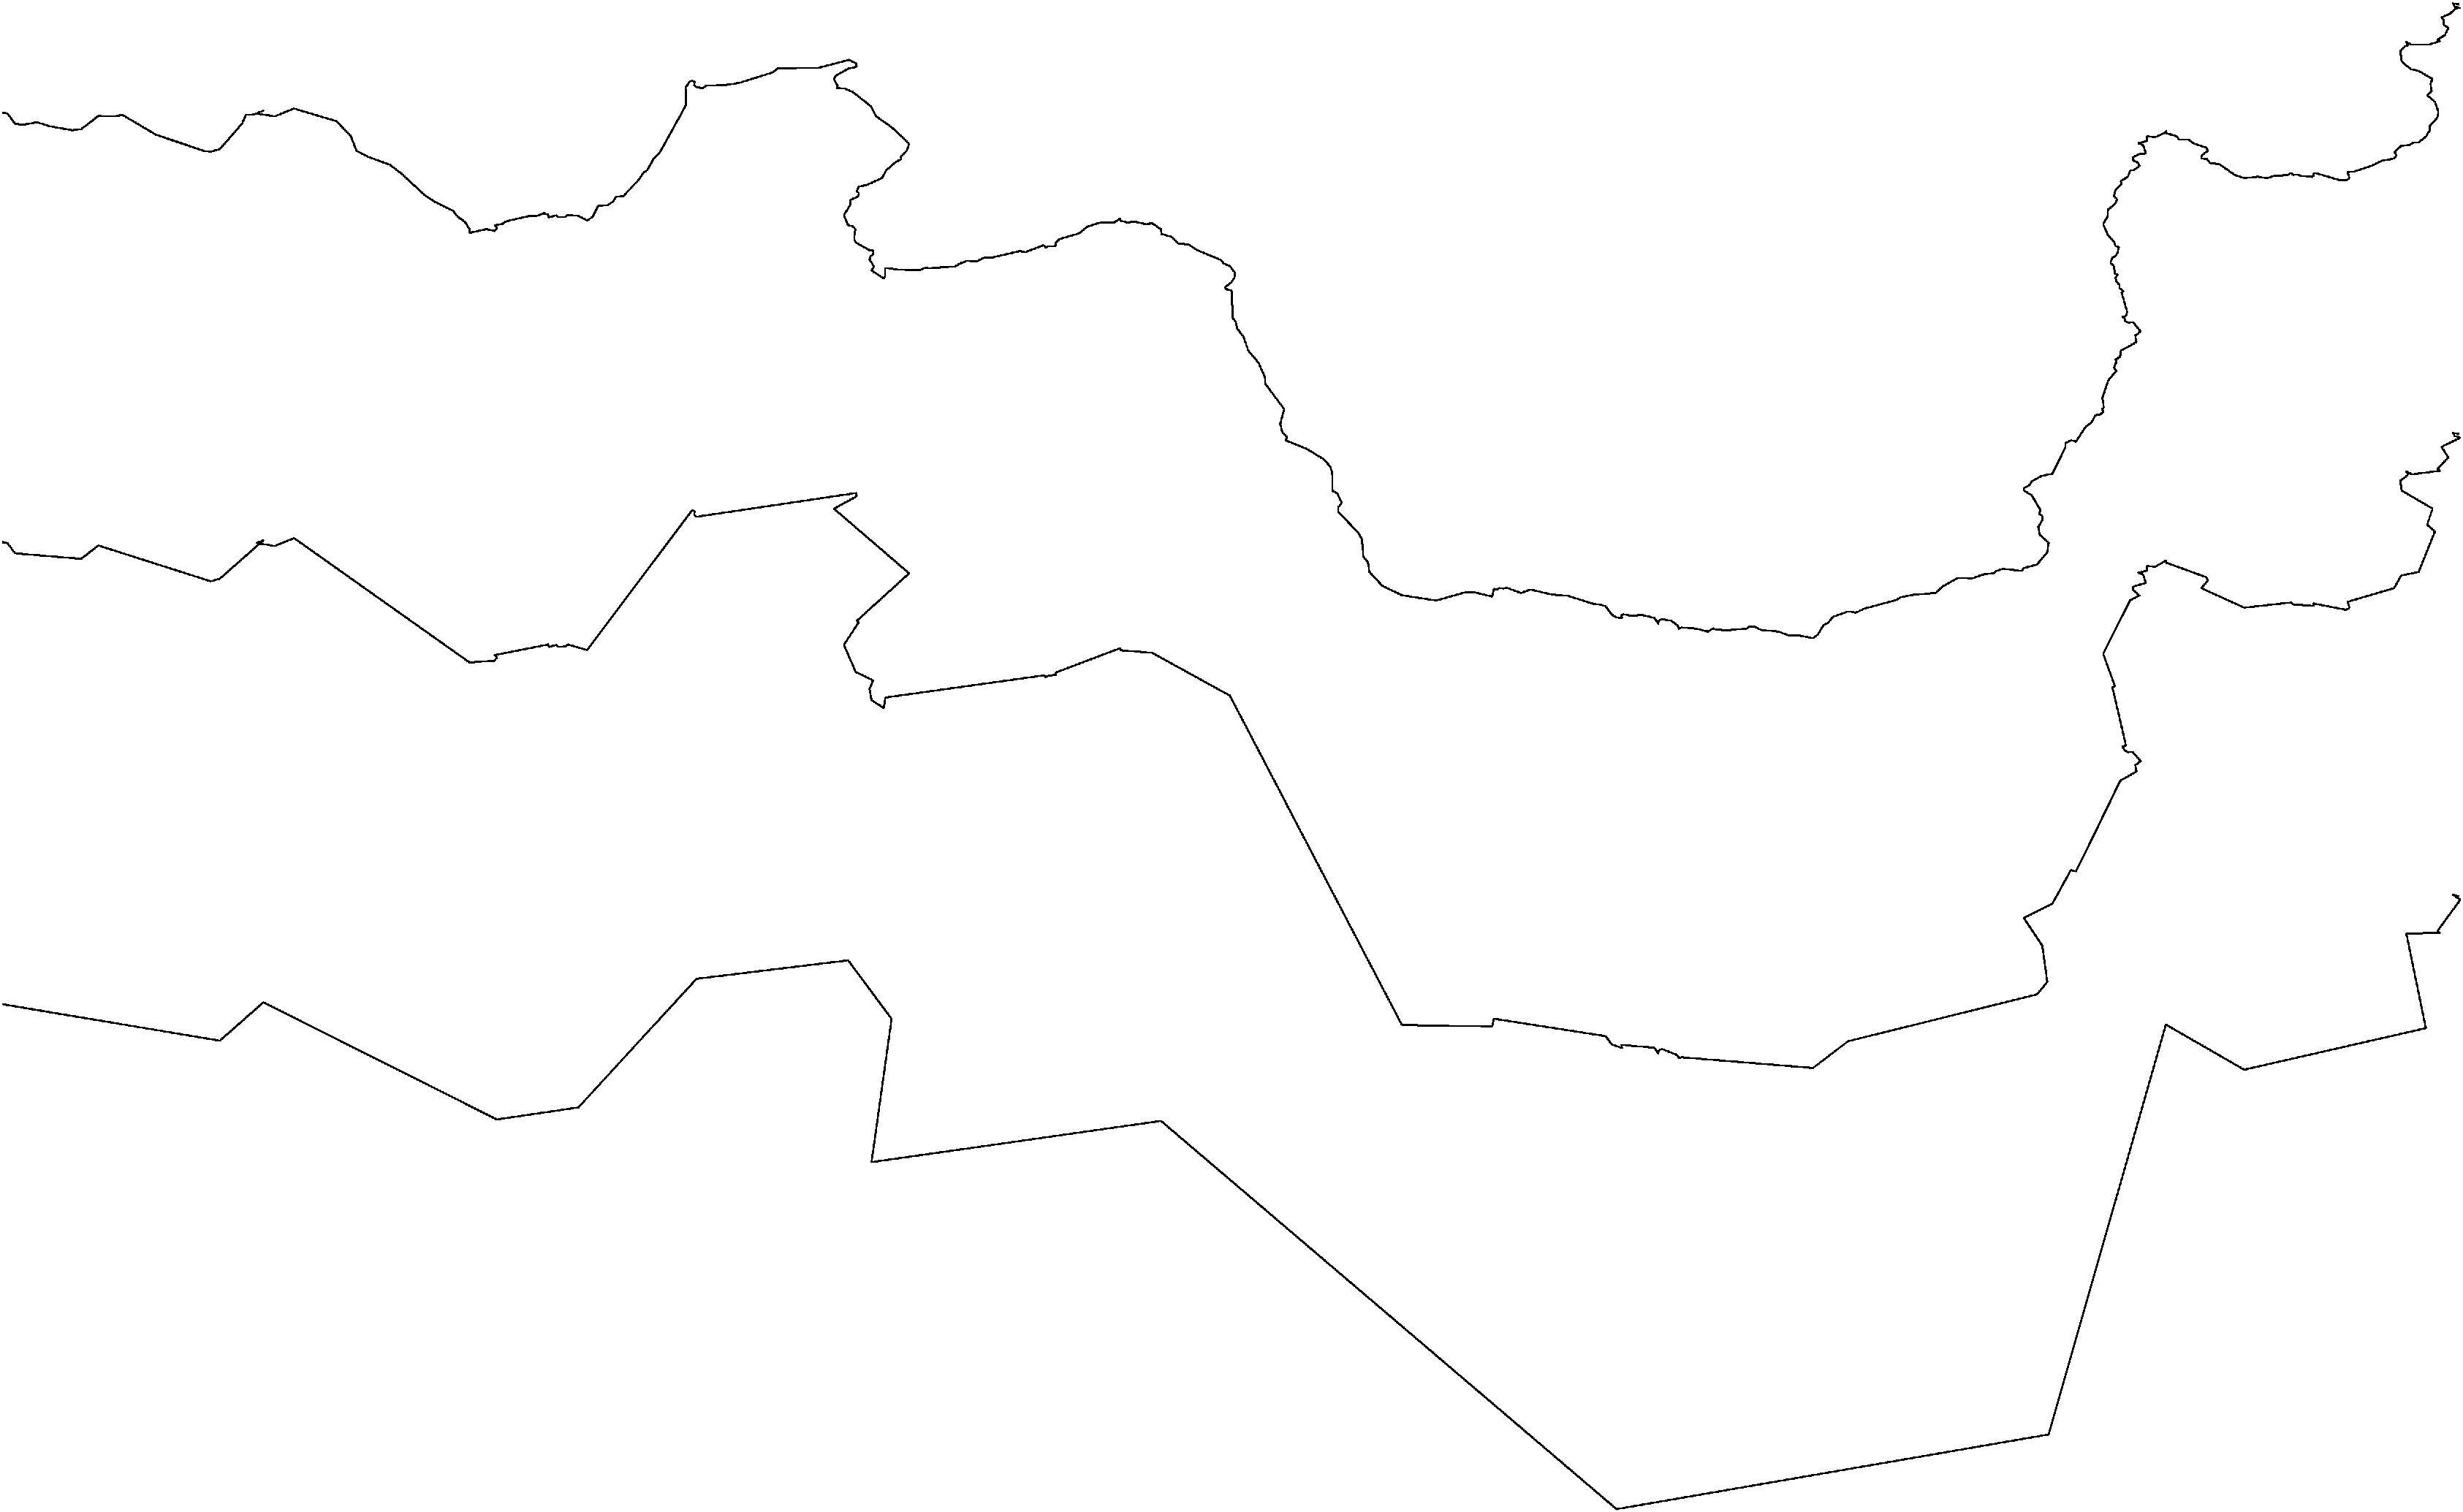
\includegraphics[scale=0.15]{approximation_example}
    	\end{minipage}
    	\caption{Kantenzug mit 430 Punkten (oben) und zwei Approximationen mit 126 bzw. 22 Punkten (mitte und unten), die aus dem approximativen Algorithmus für das MVPS-Problem mit jeweils $\epsilon = 0.05$ und $t = 1.05$ bzw. $t = 1.2$ berechnet wurden (Quelle: \cite{gudmundsson})}
    \end{figure}